\documentclass[a4paper,12pt,twocolumn]{article}

\usepackage[landscape,top=1cm,bottom=1.4cm,left=1cm,right=1cm,columnsep=1cm]{geometry}
\usepackage[fleqn]{amsmath}
\usepackage{amssymb}
\usepackage{fontspec}
\usepackage{enumitem}
\usepackage{framed}
\usepackage{needspace}
\usepackage[hidelinks]{hyperref}
\usepackage{tikz}
\usetikzlibrary{arrows.meta}

\setlength{\mathindent}{1.5em}

\setmainfont{Times New Roman}
\setsansfont{Arial}

\pagestyle{plain}
\setlength{\columnseprule}{0.2pt}

\newcommand{\examdate}{2026/05/02}
\newlength{\problemnumberwidth}
\settowidth{\problemnumberwidth}{\textbf{xiii.}\ }
\newenvironment{solutionbox}{\begin{framed}}{\end{framed}}

\newcommand{\sectiontitle}[2]{%
  \hypertarget{#1}{}%
  \phantomsection\label{#1}%
  \par\vspace{0.8em}%
  \noindent{\Large\bfseries #2}\par
  \vspace{0.3em}%
  \hrule
  \vspace{0.8em}%
}

\newcommand{\tocproblem}[2]{%
  \hyperref[#1]{#2} & \hyperref[#1]{\pageref*{#1}} \\
}

\newcommand{\worksheettoc}{%
  \noindent{\Large\bfseries Contents}\par
  \vspace{0.3em}%
  \hrule
  \vspace{0.9em}%
  \begin{tabular}{@{}p{0.72\columnwidth}r@{}}
    \textbf{Problem} & \textbf{Page} \\
    \tocproblem{prob:iv}{iv}
    \tocproblem{prob:v}{v}
    \tocproblem{prob:vi}{vi}
    \tocproblem{prob:vii}{vii}
    \tocproblem{prob:x}{x}
    \tocproblem{prob:xi}{xi}
    \tocproblem{prob:xiii}{xiii}
    \tocproblem{prob:4}{4}
    \tocproblem{prob:9}{9}
    \tocproblem{sec:final}{Final answers}
  \end{tabular}\par
}

\newcommand{\problem}[3]{%
  \Needspace{10\baselineskip}%
  \phantomsection\label{#1}%
  \par\vspace{0.8em}%
  \noindent
  \hangindent=\problemnumberwidth
  \hangafter=1
  \makebox[\problemnumberwidth][l]{\textbf{#2.}}#3\par
}

\newlist{steps}{enumerate}{1}
\setlist[steps]{%
  label=\textbf{Step \arabic*.},
  leftmargin=*,
  itemsep=0.35em,
  topsep=0.35em,
  align=left
}

\newlist{finalitems}{enumerate}{1}
\setlist[finalitems]{%
  label=\textbf{\arabic*.},
  leftmargin=*,
  itemsep=0.35em,
  topsep=0.35em,
  align=left
}

\newcommand{\roseintersectionfigure}{%
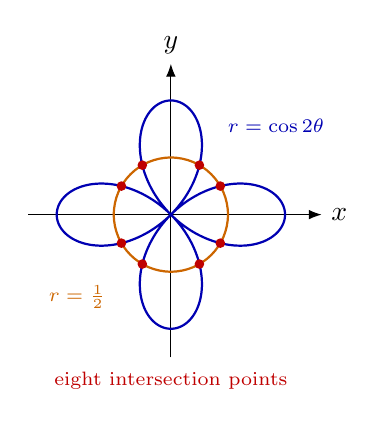
\begin{tikzpicture}[scale=1.45,>=Latex]
  \draw[->,line width=0.35pt] (-1.25,0) -- (1.32,0) node[right] {\(x\)};
  \draw[->,line width=0.35pt] (0,-1.25) -- (0,1.32) node[above] {\(y\)};

  \draw[blue!70!black,thick]
    plot[domain=0:360,samples=360,variable=\t]
      ({cos(2*\t)*cos(\t)},{cos(2*\t)*sin(\t)});
  \draw[orange!80!black,thick] (0,0) circle[radius=0.5];

  \foreach \ang in {30,60,120,150,210,240,300,330}{
    \fill[red!75!black] ({0.5*cos(\ang)},{0.5*sin(\ang)}) circle[radius=1.2pt];
  }

  \node[blue!70!black] at (0.92,0.78) {\scriptsize \(r=\cos 2\theta\)};
  \node[orange!80!black] at (-0.82,-0.72) {\scriptsize \(r=\frac12\)};
  \node[red!75!black] at (0,-1.45) {\scriptsize eight intersection points};
\end{tikzpicture}%
}

\newcommand{\polarshadedfigure}{%
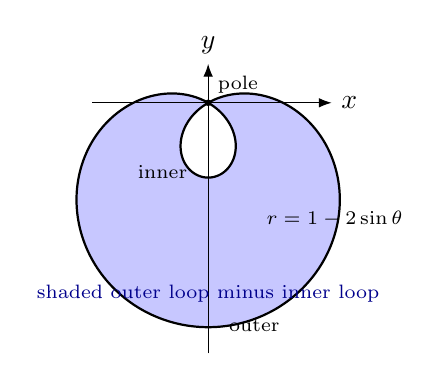
\begin{tikzpicture}[x=0.95cm,y=0.95cm,>=Latex]
  \fill[blue!22]
    plot[domain=150:390,samples=260,variable=\t]
      ({(1 - 2*sin(\t))*cos(\t)}, {(1 - 2*sin(\t))*sin(\t)})
    -- cycle;
  \fill[white]
    plot[domain=30:150,samples=160,variable=\t]
      ({(1 - 2*sin(\t))*cos(\t)}, {(1 - 2*sin(\t))*sin(\t)})
    -- cycle;

  \draw[->,line width=0.35pt] (-1.55,0) -- (1.65,0) node[right] {\(x\)};
  \draw[->,line width=0.35pt] (0,-3.35) -- (0,0.52) node[above] {\(y\)};

  \draw[black,thick]
    plot[domain=150:390,samples=260,variable=\t]
      ({(1 - 2*sin(\t))*cos(\t)}, {(1 - 2*sin(\t))*sin(\t)});
  \draw[black,thick]
    plot[domain=30:150,samples=160,variable=\t]
      ({(1 - 2*sin(\t))*cos(\t)}, {(1 - 2*sin(\t))*sin(\t)});

  \fill (0,0) circle[radius=1.2pt] node[above right] {\scriptsize pole};
  \node[right] at (0.65,-1.55) {\scriptsize \(r=1-2\sin\theta\)};
  \node[blue!55!black] at (0,-2.55) {\scriptsize shaded outer loop minus inner loop};
  \node[left] at (-0.15,-0.92) {\scriptsize inner};
  \node[right] at (0.15,-2.98) {\scriptsize outer};
\end{tikzpicture}%
}

\begin{document}

\twocolumn[
{\centering
\Large\bfseries Calculus Problems Solutions\par
\vspace{0.5em}
\noindent\hfill\normalsize\normalfont \examdate\par
\vspace{0.8em}
}
]

\worksheettoc
\vfill\null
\newpage

\sectiontitle{sec:midterm}{Midterm Problems}

\problem{prob:iv}{iv}{The series
\[
\sum_{n=1}^{\infty}\frac{\cos(n\pi)}{n}
\]
is absolutely convergent, conditionally convergent, or divergent.}

\begin{solutionbox}
\textbf{Method 1: Alternating-series test plus absolute test}

\begin{steps}
\item Since
\[
\cos(n\pi)=(-1)^n,
\]
the series becomes
\[
\sum_{n=1}^{\infty}\frac{(-1)^n}{n}.
\]
This rewrite is appropriate because the only changing part of the numerator is the sign, and identifying the sign pattern tells us which convergence test fits naturally.

\item Check absolute convergence:
\[
\sum_{n=1}^{\infty}\left|\frac{(-1)^n}{n}\right|
=\sum_{n=1}^{\infty}\frac1n.
\]
This is the harmonic series, and it diverges. Therefore the original series cannot be absolutely convergent.

\item Now check ordinary convergence. The terms \(1/n\) are positive, decrease to \(0\), and the signs alternate. Those are exactly the hypotheses of the alternating-series test, so
\[
\sum_{n=1}^{\infty}\frac{(-1)^n}{n}
\]
converges.

\item A series that converges but does not converge absolutely is conditionally convergent.
\end{steps}
\end{solutionbox}

\begin{solutionbox}
\textbf{Method 2: Use the known alternating harmonic sum}

\begin{steps}
\item Again use \(\cos(n\pi)=(-1)^n\), so
\[
\sum_{n=1}^{\infty}\frac{\cos(n\pi)}{n}
=\sum_{n=1}^{\infty}\frac{(-1)^n}{n}.
\]
This puts the problem into the standard alternating harmonic form.

\item The Taylor series
\[
\ln(1+x)=\sum_{n=1}^{\infty}\frac{(-1)^{n-1}x^n}{n}
\]
gives, at \(x=1\),
\[
\ln 2=\sum_{n=1}^{\infty}\frac{(-1)^{n-1}}{n}.
\]
Thus the given series equals \(-\ln 2\), so it is convergent.

\item However, taking absolute values gives \(\sum 1/n\), which diverges. This separates ordinary convergence from absolute convergence.
\end{steps}

\textbf{Hand-in Version.}
\[
\sum_{n=1}^{\infty}\frac{\cos(n\pi)}{n}
=\sum_{n=1}^{\infty}\frac{(-1)^n}{n}
\]
converges by the alternating-series test, but
\[
\sum_{n=1}^{\infty}\left|\frac{(-1)^n}{n}\right|
=\sum_{n=1}^{\infty}\frac1n
\]
diverges. Therefore the series is
\[
\boxed{\text{conditionally convergent}}
\]
which is choice \(\boxed{\text{B}}\).
\end{solutionbox}

\problem{prob:v}{v}{The series
\[
\sum_{n=1}^{\infty}(-1)^n\frac{100^n}{n!}
\]
is absolutely convergent, conditionally convergent, or divergent.}

\begin{solutionbox}
\textbf{Method 1: Ratio test on the absolute-value series}

\begin{steps}
\item To decide absolute convergence, remove the signs and study
\[
\sum_{n=1}^{\infty}\frac{100^n}{n!}.
\]
This is appropriate because absolute convergence is stronger than conditional convergence, and the factorial in the denominator suggests the ratio test.

\item Let
\[
a_n=\frac{100^n}{n!}.
\]
Then
\[
\frac{a_{n+1}}{a_n}
=\frac{100^{n+1}}{(n+1)!}\cdot \frac{n!}{100^n}
=\frac{100}{n+1}.
\]

\item Taking the limit,
\[
\lim_{n\to\infty}\frac{a_{n+1}}{a_n}=0<1.
\]
The ratio test says the absolute-value series converges.

\item Since the series converges after taking absolute values, the original alternating series is absolutely convergent.
\end{steps}
\end{solutionbox}

\begin{solutionbox}
\textbf{Method 2: Recognize the exponential series}

\begin{steps}
\item The absolute-value series is
\[
\sum_{n=1}^{\infty}\frac{100^n}{n!}.
\]
This resembles the exponential series, so we compare it to
\[
e^x=\sum_{n=0}^{\infty}\frac{x^n}{n!}.
\]

\item With \(x=100\),
\[
\sum_{n=0}^{\infty}\frac{100^n}{n!}=e^{100},
\]
which is finite. The given absolute-value series starts at \(n=1\), so it equals
\[
e^{100}-1.
\]

\item Because the absolute values have a finite sum, the original series converges absolutely.
\end{steps}

\textbf{Hand-in Version.}
\[
\sum_{n=1}^{\infty}\left|(-1)^n\frac{100^n}{n!}\right|
=\sum_{n=1}^{\infty}\frac{100^n}{n!}
=e^{100}-1<\infty.
\]
Hence the series is
\[
\boxed{\text{absolutely convergent}}
\]
which is choice \(\boxed{\text{A}}\).
\end{solutionbox}

\problem{prob:vi}{vi}{Find the radius of convergence of
\[
\sum_{n=1}^{\infty}\frac{(x+1)^n}{\sqrt n\,3^n}.
\]}

\begin{solutionbox}
\textbf{Method 1: Ratio test}

\begin{steps}
\item Use the absolute-value form
\[
a_n=\left|\frac{(x+1)^n}{\sqrt n\,3^n}\right|.
\]
The ratio test is appropriate because each term contains an \(n\)-th power and a neighboring factorial-like factor \(\sqrt n\).

\item Compute the ratio:
\[
\frac{a_{n+1}}{a_n}
=\frac{|x+1|^{n+1}}{\sqrt{n+1}\,3^{n+1}}
\cdot
\frac{\sqrt n\,3^n}{|x+1|^n}
=\frac{|x+1|}{3}\sqrt{\frac{n}{n+1}}.
\]

\item Let \(n\to\infty\):
\[
\lim_{n\to\infty}\frac{a_{n+1}}{a_n}
=\frac{|x+1|}{3}.
\]
The ratio test gives convergence when
\[
\frac{|x+1|}{3}<1,
\]
or
\[
|x+1|<3.
\]

\item A power series centered at \(-1\) that converges for \(|x+1|<3\) has radius of convergence \(3\). Endpoint behavior does not change the radius.
\end{steps}
\end{solutionbox}

\begin{solutionbox}
\textbf{Method 2: Root test}

\begin{steps}
\item The root test is natural for power series because it removes the \(n\)-th power. Start with
\[
a_n=\left|\frac{(x+1)^n}{\sqrt n\,3^n}\right|.
\]

\item Take the \(n\)-th root:
\[
\sqrt[n]{a_n}
=\frac{|x+1|}{3\sqrt[n]{\sqrt n}}
=\frac{|x+1|}{3n^{1/(2n)}}.
\]

\item Since
\[
n^{1/(2n)}\to 1,
\]
we get
\[
\lim_{n\to\infty}\sqrt[n]{a_n}
=\frac{|x+1|}{3}.
\]
The root test gives convergence when this limit is less than \(1\).

\item Therefore the interval of convergence begins with \(|x+1|<3\), so the radius is \(3\).
\end{steps}

\textbf{Hand-in Version.}
\[
\lim_{n\to\infty}
\left|
\frac{(x+1)^{n+1}}{\sqrt{n+1}\,3^{n+1}}
\cdot
\frac{\sqrt n\,3^n}{(x+1)^n}
\right|
=\frac{|x+1|}{3}.
\]
Thus the series converges for \(|x+1|<3\). The radius of convergence is
\[
\boxed{3}
\]
which is choice \(\boxed{\text{D}}\).
\end{solutionbox}

\problem{prob:vii}{vii}{Find the radius of convergence of
\[
\sum_{n=0}^{\infty}(2n)!\,x^{2n}.
\]}

\begin{solutionbox}
\textbf{Method 1: Ratio test}

\begin{steps}
\item Let
\[
a_n=(2n)!\,|x|^{2n}.
\]
The ratio test is appropriate because factorials grow very quickly, and the ratio of consecutive factorial terms simplifies exactly.

\item Compute
\[
\frac{a_{n+1}}{a_n}
=\frac{(2n+2)!\,|x|^{2n+2}}{(2n)!\,|x|^{2n}}
=(2n+2)(2n+1)|x|^2.
\]

\item If \(x\ne0\), then
\[
(2n+2)(2n+1)|x|^2\to\infty.
\]
So the terms grow too fast for convergence; in particular, the series cannot converge for any nonzero \(x\).

\item If \(x=0\), then all terms after the first are \(0\), so the series converges. Therefore the only point of convergence is \(x=0\), and the radius of convergence is \(0\).
\end{steps}
\end{solutionbox}

\begin{solutionbox}
\textbf{Method 2: Treat it as a power series in \(y=x^2\)}

\begin{steps}
\item Set
\[
y=x^2.
\]
Then the series becomes
\[
\sum_{n=0}^{\infty}(2n)!\,y^n.
\]
This substitution is appropriate because the original series contains only even powers of \(x\).

\item For a power series \(\sum c_n y^n\), the radius in \(y\) is
\[
R_y=\frac{1}{\limsup\limits_{n\to\infty}|c_n|^{1/n}}.
\]
Here \(c_n=(2n)!\).

\item Since factorial growth is faster than any exponential growth,
\[
\lim_{n\to\infty}((2n)!)^{1/n}=\infty.
\]
Thus
\[
R_y=0.
\]

\item The condition \(|y|<0\) leaves only \(y=0\), which means \(x^2=0\), or \(x=0\). Hence the radius in \(x\) is also \(0\).
\end{steps}

\textbf{Hand-in Version.}
\[
\frac{(2n+2)!\,|x|^{2n+2}}{(2n)!\,|x|^{2n}}
=(2n+2)(2n+1)|x|^2.
\]
For every \(x\ne0\), this ratio goes to \(\infty\), so the series diverges. It converges only at \(x=0\). Therefore the radius of convergence is
\[
\boxed{0}
\]
which is choice \(\boxed{\text{A}}\).
\end{solutionbox}

\problem{prob:x}{x}{Find the sum of
\[
\sum_{k=1}^{\infty}\frac{1}{k(k+2)}.
\]}

\begin{solutionbox}
\textbf{Method 1: Partial fractions and telescoping}

\begin{steps}
\item Decompose the term:
\[
\frac{1}{k(k+2)}
=\frac12\left(\frac1k-\frac{1}{k+2}\right).
\]
This is appropriate because the denominator has two linear factors separated by \(2\), which often creates cancellation in a series.

\item Write the \(N\)-th partial sum:
\[
S_N=\frac12\sum_{k=1}^{N}\left(\frac1k-\frac{1}{k+2}\right).
\]

\item Expand enough terms to see the cancellation:
\[
S_N=\frac12\left(1+\frac12+\frac13+\cdots+\frac1N
-\frac13-\frac14-\cdots-\frac1{N+2}\right).
\]
All middle terms cancel because each \(\frac1j\) for \(3\le j\le N\) appears once with a plus sign and once with a minus sign.

\item The remaining terms are
\[
S_N=\frac12\left(1+\frac12-\frac1{N+1}-\frac1{N+2}\right).
\]
Letting \(N\to\infty\),
\[
S=\frac12\left(1+\frac12\right)=\frac34.
\]
\end{steps}
\end{solutionbox}

\begin{solutionbox}
\textbf{Method 2: Integral form and geometric series}

\begin{steps}
\item Use the identity
\[
\frac{1}{k(k+2)}
=\frac12\left(\frac1k-\frac{1}{k+2}\right)
=\frac12\int_0^1\left(x^{k-1}-x^{k+1}\right)\,dx.
\]
This is useful because integrals of powers produce the factors \(1/k\) and \(1/(k+2)\).

\item Sum over \(k\):
\[
\sum_{k=1}^{\infty}\frac{1}{k(k+2)}
=\frac12\int_0^1\sum_{k=1}^{\infty}\left(x^{k-1}-x^{k+1}\right)\,dx.
\]
The terms are controlled on \(0\le x<1\), and this turns the series into a geometric series.

\item Inside the integral,
\[
\sum_{k=1}^{\infty}\left(x^{k-1}-x^{k+1}\right)
=(1-x^2)\sum_{k=1}^{\infty}x^{k-1}
=(1-x^2)\frac{1}{1-x}.
\]
Since
\[
\frac{1-x^2}{1-x}=1+x,
\]
the integral becomes simple.

\item Therefore
\[
\sum_{k=1}^{\infty}\frac{1}{k(k+2)}
=\frac12\int_0^1(1+x)\,dx
=\frac12\left[x+\frac{x^2}{2}\right]_0^1
=\frac34.
\]
\end{steps}

\textbf{Hand-in Version.}
\[
\frac{1}{k(k+2)}
=\frac12\left(\frac1k-\frac1{k+2}\right).
\]
Thus
\[
\sum_{k=1}^{N}\frac{1}{k(k+2)}
=\frac12\left(1+\frac12-\frac1{N+1}-\frac1{N+2}\right).
\]
Taking \(N\to\infty\),
\[
\boxed{\sum_{k=1}^{\infty}\frac{1}{k(k+2)}=\frac34}
\]
which is choice \(\boxed{\text{C}}\).
\end{solutionbox}

\problem{prob:xi}{xi}{Find the number of points of intersection of
\[
r=\cos 2\theta
\qquad\text{and}\qquad
r=\frac12.
\]}

\begin{solutionbox}
\textbf{Method 1: Solve using the polar meaning of negative \(r\)}

\begin{steps}
\item The curve \(r=\frac12\) is the circle of radius \(\frac12\) centered at the pole. Therefore a point on the rose intersects this circle exactly when its distance from the pole is \(\frac12\).

\item For the rose \(r=\cos 2\theta\), negative \(r\)-values still create points on the graph: a negative radius plots the point in the opposite direction. So the distance from the pole is
\[
|r|=|\cos 2\theta|.
\]
This step is important because solving only \(\cos 2\theta=\frac12\) would miss the points where the rose has \(r=-\frac12\).

\item Set the distance equal to \(\frac12\):
\[
|\cos 2\theta|=\frac12.
\]
Equivalently,
\[
\cos 2\theta=\frac12
\qquad\text{or}\qquad
\cos 2\theta=-\frac12.
\]

\item On \(0\le\theta<2\pi\), these equations give eight distinct plotted points on the circle:
\[
\theta=\frac{\pi}{6},\frac{\pi}{3},\frac{2\pi}{3},\frac{5\pi}{6},
\frac{7\pi}{6},\frac{4\pi}{3},\frac{5\pi}{3},\frac{11\pi}{6}
\]
after accounting for the opposite-direction plotting of negative \(r\). Hence there are \(8\) intersection points.
\end{steps}
\end{solutionbox}

\begin{solutionbox}
\textbf{Method 2: Geometric counting from the graph}

\begin{steps}
\item The equation \(r=\cos 2\theta\) is a four-petal rose. Each petal starts at the pole, reaches maximum distance \(1\), and returns to the pole.

\item The circle \(r=\frac12\) has radius \(\frac12\), which is between \(0\) and the maximum petal length \(1\). Therefore it must cross each petal once on the way out and once on the way back.

\item Since there are \(4\) petals and \(2\) crossings on each petal, the number of intersections is
\[
4\cdot 2=8.
\]
\end{steps}

\begin{center}
\roseintersectionfigure
\end{center}

\textbf{Hand-in Version.}
The circle \(r=\frac12\) intersects the four-petal rose \(r=\cos 2\theta\) twice on each petal. Therefore the number of intersection points is
\[
\boxed{8}
\]
which is choice \(\boxed{\text{D}}\).
\end{solutionbox}

\problem{prob:xiii}{xiii}{Compute
\[
\binom{1/2}{4}.
\]}

\begin{solutionbox}
\textbf{Method 1: Use the definition of generalized binomial coefficients}

\begin{steps}
\item For any real number \(\alpha\),
\[
\binom{\alpha}{4}
=\frac{\alpha(\alpha-1)(\alpha-2)(\alpha-3)}{4!}.
\]
This definition is appropriate because the top number \(1/2\) is not an integer.

\item Substitute \(\alpha=\frac12\):
\[
\binom{1/2}{4}
=\frac{\left(\frac12\right)\left(\frac12-1\right)
\left(\frac12-2\right)\left(\frac12-3\right)}{24}.
\]

\item Simplify each factor:
\[
\binom{1/2}{4}
=\frac{\left(\frac12\right)\left(-\frac12\right)
\left(-\frac32\right)\left(-\frac52\right)}{24}.
\]
There are three negative factors, so the result is negative.

\item Compute the magnitude:
\[
\frac{1\cdot1\cdot3\cdot5}{2^4\cdot24}
=\frac{15}{384}
=\frac{5}{128}
=\frac{5}{2^7}.
\]
Therefore
\[
\binom{1/2}{4}=-\frac{5}{2^7}.
\]
\end{steps}
\end{solutionbox}

\begin{solutionbox}
\textbf{Method 2: Build the coefficients recursively}

\begin{steps}
\item Use the recurrence
\[
\binom{\alpha}{m}
=\binom{\alpha}{m-1}\frac{\alpha-m+1}{m}.
\]
This method is efficient because it builds the coefficient one order at a time without rewriting the full product.

\item Start with
\[
\binom{1/2}{1}=\frac12.
\]

\item Then
\[
\binom{1/2}{2}
=\binom{1/2}{1}\frac{\frac12-1}{2}
=\frac12\cdot\frac{-1/2}{2}
=-\frac18.
\]

\item Next,
\[
\binom{1/2}{3}
=\binom{1/2}{2}\frac{\frac12-2}{3}
=-\frac18\cdot\frac{-3/2}{3}
=\frac1{16}.
\]

\item Finally,
\[
\binom{1/2}{4}
=\binom{1/2}{3}\frac{\frac12-3}{4}
=\frac1{16}\cdot\frac{-5/2}{4}
=-\frac5{128}
=-\frac5{2^7}.
\]
\end{steps}

\textbf{Hand-in Version.}
\[
\binom{1/2}{4}
=\frac{\left(\frac12\right)\left(-\frac12\right)
\left(-\frac32\right)\left(-\frac52\right)}{4!}
=-\frac{5}{128}
=\boxed{-\frac5{2^7}}.
\]
This is choice \(\boxed{\text{H}}\).
\end{solutionbox}

\problem{prob:4}{4}{Let
\[
f(x)=\frac{1}{(1-2x^2)^5}.
\]
Suppose
\[
f^{(10)}(0)=a\binom{-5}{k}2^n.
\]
Find \(a\), \(k\), and \(n\).}

\begin{solutionbox}
\textbf{Method 1: Generalized binomial series}

\begin{steps}
\item Rewrite the function as
\[
f(x)=(1-2x^2)^{-5}.
\]
The generalized binomial theorem applies because this has the form \((1+u)^\alpha\), with \(\alpha=-5\) and \(u=-2x^2\).

\item Expand:
\[
(1-2x^2)^{-5}
=\sum_{m=0}^{\infty}\binom{-5}{m}(-2x^2)^m.
\]
This is useful because derivatives at \(0\) are determined by Maclaurin coefficients.

\item The term containing \(x^{10}\) occurs when
\[
2m=10,
\]
so
\[
m=5.
\]
Thus the \(x^{10}\)-coefficient is
\[
\binom{-5}{5}(-2)^5
=-\binom{-5}{5}2^5.
\]

\item In a Maclaurin series,
\[
f(x)=\sum_{j=0}^{\infty}\frac{f^{(j)}(0)}{j!}x^j.
\]
Therefore
\[
f^{(10)}(0)=10!\cdot [x^{10}]f(x).
\]
So
\[
f^{(10)}(0)
=10!\left(-\binom{-5}{5}2^5\right)
=-10!\binom{-5}{5}2^5.
\]

\item Comparing with
\[
f^{(10)}(0)=a\binom{-5}{k}2^n,
\]
we get
\[
a=-10!,\qquad k=5,\qquad n=5.
\]
\end{steps}
\end{solutionbox}

\begin{solutionbox}
\textbf{Method 2: Use the positive-coefficient form of \((1-z)^{-5}\)}

\begin{steps}
\item The standard identity
\[
(1-z)^{-5}=\sum_{m=0}^{\infty}\binom{m+4}{4}z^m
\]
is useful here because the denominator is a fifth power and the coefficients are positive.

\item Put
\[
z=2x^2.
\]
Then
\[
f(x)=\sum_{m=0}^{\infty}\binom{m+4}{4}(2x^2)^m.
\]

\item The \(x^{10}\)-term again corresponds to \(2m=10\), so \(m=5\). Its coefficient is
\[
\binom{9}{4}2^5=\binom{9}{5}2^5.
\]

\item Since
\[
\binom{-5}{5}=(-1)^5\binom{9}{5}=-\binom{9}{5},
\]
we can rewrite the coefficient as
\[
-\binom{-5}{5}2^5.
\]
Multiplying by \(10!\) gives
\[
f^{(10)}(0)=-10!\binom{-5}{5}2^5.
\]

\item Therefore
\[
a=-10!,\qquad k=5,\qquad n=5.
\]
\end{steps}

\textbf{Hand-in Version.}
\[
(1-2x^2)^{-5}
=\sum_{m=0}^{\infty}\binom{-5}{m}(-2x^2)^m.
\]
The \(x^{10}\)-term occurs when \(m=5\), so
\[
[x^{10}]f(x)=\binom{-5}{5}(-2)^5
=-\binom{-5}{5}2^5.
\]
Thus
\[
f^{(10)}(0)=10![x^{10}]f(x)
=-10!\binom{-5}{5}2^5.
\]
Hence
\[
\boxed{a=-10!,\qquad k=5,\qquad n=5.}
\]
Equivalently, \(a=-3628800\).
\end{solutionbox}

\problem{prob:9}{9}{For the polar curve
\[
r=1-2\sin\theta,
\]
(a) find \(\dfrac{dy}{dx}\), and (b) set up the definite integral for the area of the shaded region.}

\begin{solutionbox}
\textbf{Method 1: Parametric differentiation and loop subtraction}

\begin{steps}
\item Write the polar curve in parametric form:
\[
x=r\cos\theta=(1-2\sin\theta)\cos\theta,
\]
\[
y=r\sin\theta=(1-2\sin\theta)\sin\theta.
\]
This is the correct starting point because \(\frac{dy}{dx}\) for a polar curve is found by treating both \(x\) and \(y\) as functions of \(\theta\).

\item Use
\[
\frac{dy}{dx}=\frac{dy/d\theta}{dx/d\theta}.
\]
Here
\[
r=1-2\sin\theta,
\qquad
\frac{dr}{d\theta}=-2\cos\theta.
\]
For polar curves,
\[
\frac{dy}{d\theta}=r'\sin\theta+r\cos\theta,
\]
\[
\frac{dx}{d\theta}=r'\cos\theta-r\sin\theta.
\]
These formulas come directly from the product rule applied to \(y=r\sin\theta\) and \(x=r\cos\theta\).

\item Substitute \(r=1-2\sin\theta\) and \(r'=-2\cos\theta\):
\[
\frac{dy}{d\theta}
=(-2\cos\theta)\sin\theta+(1-2\sin\theta)\cos\theta
=\cos\theta(1-4\sin\theta),
\]
and
\[
\frac{dx}{d\theta}
=(-2\cos\theta)\cos\theta-(1-2\sin\theta)\sin\theta
=4\sin^2\theta-\sin\theta-2.
\]

\item Therefore
\[
\frac{dy}{dx}
=\boxed{\frac{\cos\theta(1-4\sin\theta)}
{4\sin^2\theta-\sin\theta-2}}.
\]
The denominator is \(dx/d\theta\), so values where it is \(0\) correspond to vertical tangents rather than ordinary finite slopes.

\item For the area, first find where the curve meets the pole:
\[
1-2\sin\theta=0
\quad\Longrightarrow\quad
\sin\theta=\frac12.
\]
So
\[
\theta=\frac{\pi}{6},\frac{5\pi}{6}.
\]
These values matter because they separate the inner loop from the outer loop.

\item On
\[
\frac{\pi}{6}\le\theta\le\frac{5\pi}{6},
\]
the curve traces the inner loop. The outer loop is traced from
\[
\theta=\frac{5\pi}{6}
\quad\text{to}\quad
\theta=\frac{13\pi}{6}.
\]
This choice starts at the pole, travels around the large loop, and returns to the pole.

\item The polar area formula is
\[
A=\frac12\int_{\alpha}^{\beta}r^2\,d\theta.
\]
The shaded region is the large outer loop with the small inner loop removed, so
\[
A
=\frac12\int_{5\pi/6}^{13\pi/6}(1-2\sin\theta)^2\,d\theta
-\frac12\int_{\pi/6}^{5\pi/6}(1-2\sin\theta)^2\,d\theta.
\]
\end{steps}
\end{solutionbox}

\begin{solutionbox}
\textbf{Method 2: Polar tangent geometry and symmetry}

\begin{steps}
\item For a polar curve, the tangent vector has a radial part \(r'\) and an angular part \(r\). Thus the angle \(\phi\) between the tangent line and the radial direction satisfies
\[
\tan\phi=\frac{r}{r'}.
\]
This is useful because the slope angle measured from the positive \(x\)-axis is \(\theta+\phi\).

\item Therefore
\[
\frac{dy}{dx}=\tan(\theta+\phi)
=\frac{\tan\theta+\tan\phi}{1-\tan\theta\tan\phi}
=\frac{\tan\theta+\frac{r}{r'}}
{1-\tan\theta\frac{r}{r'}}.
\]
Multiplying numerator and denominator by \(r'\cos\theta\) gives the standard polar slope formula
\[
\frac{dy}{dx}
=\frac{r'\sin\theta+r\cos\theta}{r'\cos\theta-r\sin\theta}.
\]

\item Substitute
\[
r=1-2\sin\theta,
\qquad
r'=-2\cos\theta.
\]
This gives
\[
\frac{dy}{dx}
=\frac{\cos\theta(1-4\sin\theta)}
{4\sin^2\theta-\sin\theta-2}.
\]

\item For the shaded area, use symmetry about the \(y\)-axis. The right half of the outer loop is traced by
\[
\frac{3\pi}{2}\le\theta\le\frac{13\pi}{6},
\]
and the right half of the inner loop is traced by
\[
\frac{\pi}{2}\le\theta\le\frac{5\pi}{6}.
\]
This works because the curve is symmetric about the vertical axis, so the whole shaded area is twice the right-half area.

\item Thus an equivalent setup is
\[
A
=2\left[
\frac12\int_{3\pi/2}^{13\pi/6}(1-2\sin\theta)^2\,d\theta
-\frac12\int_{\pi/2}^{5\pi/6}(1-2\sin\theta)^2\,d\theta
\right].
\]
This is the same shaded region as in Method 1, just counted by symmetry.
\end{steps}

\begin{center}
\polarshadedfigure
\end{center}

\textbf{Hand-in Version.}
For \(r=1-2\sin\theta\),
\[
r'=-2\cos\theta.
\]
So
\[
\frac{dy}{dx}
=\frac{r'\sin\theta+r\cos\theta}{r'\cos\theta-r\sin\theta}
=\boxed{\frac{\cos\theta(1-4\sin\theta)}
{4\sin^2\theta-\sin\theta-2}}.
\]

The pole occurs when
\[
1-2\sin\theta=0,
\]
so \(\theta=\pi/6,5\pi/6\). The inner loop is traced on
\[
\left[\frac{\pi}{6},\frac{5\pi}{6}\right],
\]
and the outer loop is traced on
\[
\left[\frac{5\pi}{6},\frac{13\pi}{6}\right].
\]
Therefore the shaded area is set up as
\[
\boxed{
A
=\frac12\int_{5\pi/6}^{13\pi/6}(1-2\sin\theta)^2\,d\theta
-\frac12\int_{\pi/6}^{5\pi/6}(1-2\sin\theta)^2\,d\theta.
}
\]
If evaluated, this area is
\[
A=\pi+3\sqrt3.
\]
\end{solutionbox}

\sectiontitle{sec:final}{Final Hand-in Answers}

\begin{solutionbox}
\begin{finalitems}
\item[\textbf{iv.}] \(\displaystyle \sum_{n=1}^{\infty}\frac{\cos(n\pi)}{n}\) is
\[
\boxed{\text{conditionally convergent}}\qquad(\text{B}).
\]

\item[\textbf{v.}] \(\displaystyle \sum_{n=1}^{\infty}(-1)^n\frac{100^n}{n!}\) is
\[
\boxed{\text{absolutely convergent}}\qquad(\text{A}).
\]

\item[\textbf{vi.}] \(\displaystyle \sum_{n=1}^{\infty}\frac{(x+1)^n}{\sqrt n\,3^n}\) has radius of convergence
\[
\boxed{3}\qquad(\text{D}).
\]

\item[\textbf{vii.}] \(\displaystyle \sum_{n=0}^{\infty}(2n)!\,x^{2n}\) has radius of convergence
\[
\boxed{0}\qquad(\text{A}).
\]

\item[\textbf{x.}] \(\displaystyle \sum_{k=1}^{\infty}\frac{1}{k(k+2)}\) has sum
\[
\boxed{\frac34}\qquad(\text{C}).
\]

\item[\textbf{xi.}] The curves \(r=\cos 2\theta\) and \(r=\frac12\) have
\[
\boxed{8}
\]
points of intersection, choice \(\boxed{\text{D}}\).

\item[\textbf{xiii.}]
\[
\binom{1/2}{4}
=\boxed{-\frac5{2^7}}
\]
which is choice \(\boxed{\text{H}}\).

\item[\textbf{4.}] For \(f(x)=(1-2x^2)^{-5}\),
\[
f^{(10)}(0)=-10!\binom{-5}{5}2^5,
\]
so
\[
\boxed{a=-10!,\qquad k=5,\qquad n=5.}
\]

\item[\textbf{9.}] For \(r=1-2\sin\theta\),
\[
\boxed{\frac{dy}{dx}
=\frac{\cos\theta(1-4\sin\theta)}
{4\sin^2\theta-\sin\theta-2}}.
\]
The shaded area is
\[
\boxed{
A
=\frac12\int_{5\pi/6}^{13\pi/6}(1-2\sin\theta)^2\,d\theta
-\frac12\int_{\pi/6}^{5\pi/6}(1-2\sin\theta)^2\,d\theta
}
\]
and, if evaluated,
\[
\boxed{A=\pi+3\sqrt3.}
\]
\end{finalitems}
\end{solutionbox}

\end{document}
